\documentclass[a4paper,10pt,oneside]{article}
\usepackage[polutonikogreek,italian]{babel}
\usepackage[utf8x]{inputenc}
\usepackage{amsmath}
\usepackage{amsthm}
\usepackage{amssymb}
\usepackage{amscd}
\usepackage{graphicx}
\usepackage{float}
\usepackage{array}
\usepackage{rotating}
\usepackage[small]{caption}
\usepackage{lscape}
\usepackage{fancybox}
\usepackage{booktabs}
\parindent0ex 
\renewcommand{\fboxsep}{0.5cm}
\usepackage{hyperref}
\renewcommand{\textfraction}{0.05}
\renewcommand{\topfraction}{0.95}
\renewcommand{\bottomfraction}{0.95}
\renewcommand{\floatpagefraction}{0.35}
\setcounter{totalnumber}{5}
\restylefloat{figure}
\newlength{\drop}
\begin{document}

\begin{center}
{\huge Laboratorio di acustica}
\end{center}

\begin{abstract}
In questo laboratorio ripeteremo l'esperimento di Kundt del 1866\footnote{L'articolo originale è stato pubblicato su\emph{Annalen der Physik} (Leipzig: J. C. Poggendorff) 127 (4): p.497–523. ed è disponibile gratuitamente su \url{http://books.google.com}} avvalendoci di una strumentazione più moderna che ci permetterà di effettuare delle osservazioni e delle misure impossibili ai tempi dello sperimentatore originale. Durante il laboratorio misureremo la velocità del suono, la lunghezza acustica di un tubo e la disposizione spaziale delle striature che si vengono a formare nella polvere di sughero a causa della risonanza.  
\end{abstract}

\vspace{3cm}

Per effettuare l'esperimento ci avverremo di 4 tubi, presenti in laboratorio, 2 opachi e due trasparenti. Tramite i tubi opachi misureremo la velocità del suono mentre quelli trasparenti verranno utilizzati per osservare le striature nella polvere di sughero.

\section{Breve richiamo teorico}

Durante questo laboratorio genereremo delle onde stazionarie che, come avete già studiato, nascono dall'interferenza costruttiva di due onde progressive con velocità opposte, nel nostro caso un'onda incidente generata da un altoparlante ed un onda riflessa dalle estremità del tubo. 

Considereremo due casi:
\begin{itemize}
 \item Tubo aperto
\item Tubo semichiuso
\end{itemize}

Prendiamo come esempio il tubo semichiuso:
\begin{figure}[H]
 \centering
 \includegraphics[width=1.1\textwidth]{../Immagini/tubo_semichiuso.png}
 % tubo_semichiuso.png: 2746x1564 pixel, 304dpi, 22.95x13.07 cm, bb=
 \caption{Onda stazionaria all'interno di un tubo semichiuso}
 \label{fig:tubo_semichiuso}
\end{figure}
vediamo che all'estremità chiusa l'onda sonora si riflette senza cambiamenti di fase mentre all'estremità aperta vi è un cambiamento di fase di $\pi$. La diversa riflessione dell'onda da parte dell'estremità aperta e di quella chiusa è la causa delle differenti frequenze risonanti nei due casi.
\subsection{Tubo aperto}

Ricordiamo che nel tubo aperto le lunghezze d'onda per cui un tubo  di lunghezza $L$ risuona sono date da:
\begin{equation}\label{aperto_1}
 \lambda_k=\frac{2L}{k}\qquad k=1,2,3...
\end{equation}

mentre per una data lunghezza d'onda $\lambda$ le lunghezze risonanti saranno:
\begin{equation}\label{aperto_2}
 L_k=k\frac{\lambda}{2}\qquad k=1,2,3... 
\end{equation}

ovvero utilizzando la relazione $\lambda=v/\nu$ possiamo riscrivere le relazioni [\ref{aperto_1}] e [\ref{aperto_2}] come:
\begin{equation}
 \nu_k=k\frac{v}{2L}
\end{equation}
e
\begin{equation}
 L_k=k\frac{v}{2\nu}
\end{equation}

Utilizzando un tubo aperto della lunghezza di $0.60m$ otteniamo teoricamente\footnote{Si può dimostrare che un tubo aperto si comporta come se fosse più lungo al fine della determinazione della frequenza risonante} le seguenti frequenze risonanti:


\begin{table}[H]
\begin{center}
\begin{tabular}{lll}\toprule
$Armonica$ &$k$&$\nu$\\ \midrule
Prima & 1 & 283Hz\\
Seconda & 2&567Hz\\
Terza & 3&851Hz\\
\ldots &\ldots&\ldots \\ \bottomrule
\end{tabular}\caption{Le frequenze sono state calcolate utilizzando per la velocità del suono in aria il valore $340.0ms^{-1}$}\label{tab:aperto}
\end{center}
\end{table}


\begin{figure}[H]
 \centering
 \includegraphics[width=\textwidth]{../Immagini/aperto_1.png}
 % aperto_1.png: 696x234 pixel, 90dpi, 19.64x6.60 cm, bb=
 \caption{Armonica fondamentale del tubo aperto, nella figura è rappresentata l'onda di spostamento notiamo la presenza di un unico nodo al centro}
 \label{fig:aperto_fondamentale}
\end{figure}

\begin{figure}[H]
 \centering
 \includegraphics[width=\textwidth]{../Immagini/aperto_2.png}
 % aperto_2.png: 696x238 pixel, 90dpi, 19.64x6.72 cm, bb=
 \caption{Seconda armonica nel tubo aperto, nella figura è rappresentata l'onda di spostamento. Notiamo la presenza di due nodi}
 \label{fig:aperto_seconda}
\end{figure}



\subsection{Tubo semichiuso}

Le frequenze risonanti per il tubo semichiuso sono diverse e risultano:
\begin{equation}\label{chiuso_1}
 \lambda_k=\frac{4L}{2k+1}\qquad k=0,1,2..
\end{equation}

mentre per una lunghezza d'onda data:
\begin{equation}\label{chiuso_2}
 L_k=(2k+1)\frac{\lambda}{4}\qquad k=0,1,2..
\end{equation}

esprimendo le relazioni [\ref{chiuso_1}] e [\ref{chiuso_2}] in funzione delle frequenza otteniamo:

\begin{equation}
 \nu_k=(2k+1)\frac{v}{4L}
\end{equation}

e
\begin{equation}
 L_k=(2k+1)\frac{v}{\nu}
\end{equation}


utilizzando un tubo semichiuso della lunghezza di $0.60m$\footnote{Anche in questo caso le frequenze calcolate con questa formula sono unicamente dei valori approssimati} otteniamo ad esempio le frequenze risonanti:
\begin{table}[H]
\begin{center}
\begin{tabular}{lll}\toprule
$Armonica$ &$k$&$\nu$\\ \midrule
Prima & 0 & 142Hz\\
Seconda & 1&425Hz\\
Terza & 2&568Hz\\
\ldots &\ldots&\ldots \\ \bottomrule
\end{tabular}\caption{Le frequenze sono state calcolate utilizzando per la velocità del suono in aria il valore $340.0ms^{-1}$}\label{tab:chiuso}
\end{center}
\end{table}

\begin{figure}[H]
 \centering
 \includegraphics[width=\textwidth]{../Immagini/chiuso_1.png}
 % chiuso_1.png: 706x240 pixel, 90dpi, 19.93x6.77 cm, bb=
 \caption{Armonica fondamentale del tubo semichiuso, nella figura è rappresentata l'onda di spostamento notiamo la presenza di un nodo}
 \label{fig:chiuso_base}
\end{figure}

\begin{figure}[H]
 \centering
 \includegraphics[width=\textwidth]{../Immagini/chiuso_2.png}
 % chiuso_2.png: 704x234 pixel, 90dpi, 19.87x6.60 cm, bb=
 \caption{Seconda armonica del tubo semichiuso, notiamo la presenza di due nodi. In figura è rappresentata l'onda di spostamento}
 \label{fig:chiuso_seconda}
\end{figure}


\subsection{Calcolo della velocità del suono}
Utilizzando le formule per il tubo semichiuso possiamo misurare in maniera estremamente semplice la velocità del suono. Calcoliamo la differenza tra due lunghezze risonanti ad una data frequenza $\lambda$:
\begin{equation}
 L_{k+1}-L_k=[2(k+1)+1]\frac{\lambda}{4}-(2k+1)\frac{\lambda}{4}=\lambda/2
\end{equation}
misurando due di tali lunghezze successive ad una data frequenza possiamo quindi ottenere il valore di mezza lunghezza d'onda.
Ricordando che:
\begin{equation}
 \lambda=vT
\end{equation}
dove $T$ è il periodo dell'onda:
\begin{equation}
 T=\frac{1}{\nu}
\end{equation}
possiamo ricavare:
\begin{equation}
 v=\lambda\nu
\end{equation}
ed ottenere la velocità del suono. Possiamo confrontare il valore misurato in laboratorio con il valore calcolato della velocità del suono in funzione della temperatura secondo la formula seguente:
\begin{equation}
 v\sim 331.3\sqrt{\frac{T}{T_0}}\ ms^{-1}
\end{equation}
dove $T$ è la temperatura ambiente in Kelvin e $T_0=273,15K$.
 

\subsection{Correzione per la lunghezza acustica}

La trattazione teorica elementare non tiene conto del fatto che la riflessione dell'onda sonora da parte dell'estremità aperta non è completa e che l'aria che esce dal tubo tende ad espandersi. Per questi motivi è estremamente facile accorgersi durante la sessione di laboratorio che le formule sopra citate non sono corrette, precisamente nel caso reale il tubo si comporta come se fosse leggermente più lungo per cui nel caso del tubo semichiuso avremo:


\begin{equation}
 L_k+\delta=(2k+1)\frac{\lambda}{4}
\end{equation}

mentre nel caso del tubo aperto:
\begin{equation}
 L_k+2\delta=k\frac{\lambda}{2}
\end{equation}

è possibile calcolare (Levine  e Schwinger, 1948) un valore per $\delta$ in funzione del diametro del tubo, tale calcolo è sfortunatamente estremamente complesso e non eseguibile con gli strumenti matematici disponibili alle scuole superiori. 
Durante l'esperimento dovremmo riuscire a misurare un valore prossimo a:
\begin{equation}
 \delta\sim 0.65r
\end{equation}

dove $r$ è il raggio del tubo.

\subsection{Striature nella polvere di sughero}

Sin dai primi esperimenti di Kundt si notò come all'instaurarsi di un'onda progressiva all'interno del tubo comparissero delle striature nella polvere utilizzata per visualizzare i nodi e i ventri del modo risonante. L'origine di tali striature eluse per quasi 70 anni la comunità scientifica. Fu soltanto nella seconda metà del XX secolo che, con il diffondersi di sistemi più sofisticati per la raccolta dei dati, il fenomeno venne interpretato correttamente\footnote{C.Andreade Trans. Roy. Soc. (London) A230, 413 (1932) l'articolo originale è disponibile in biblioteca o sulla pagina web dedicata a questo esperimento all'indirizzo \url{http://cartan.e-moka.net}}.

\begin{figure}[H]
 \centering
 \includegraphics[width=\textwidth]{../Immagini/cork1.png}
 % cork1.png: 837x334 pixel, 90dpi, 23.62x9.43 cm, bb=
 \caption{Striature nella polvere di sughero}
 \label{fig:cork1}
\end{figure}

\begin{figure}[H]
 \centering
 \includegraphics[width=\textwidth]{../Immagini/cork2.png}
 % cork2.png: 1140x363 pixel, 90dpi, 32.18x10.25 cm, bb=
 \caption{Rappresentazione dei vortici che generano le striature all'interno del tubo di Kundt}
 \label{fig:cork2}
\end{figure}

Empiricamente si è visto che la separazione $S$ tra due striature alla distanza $y$ da un ventre segue la regola:
\begin{equation}
 S=0.422\cos^{0.44}(2\pi y/\lambda)
\end{equation}


\begin{figure}[H]
 \centering
 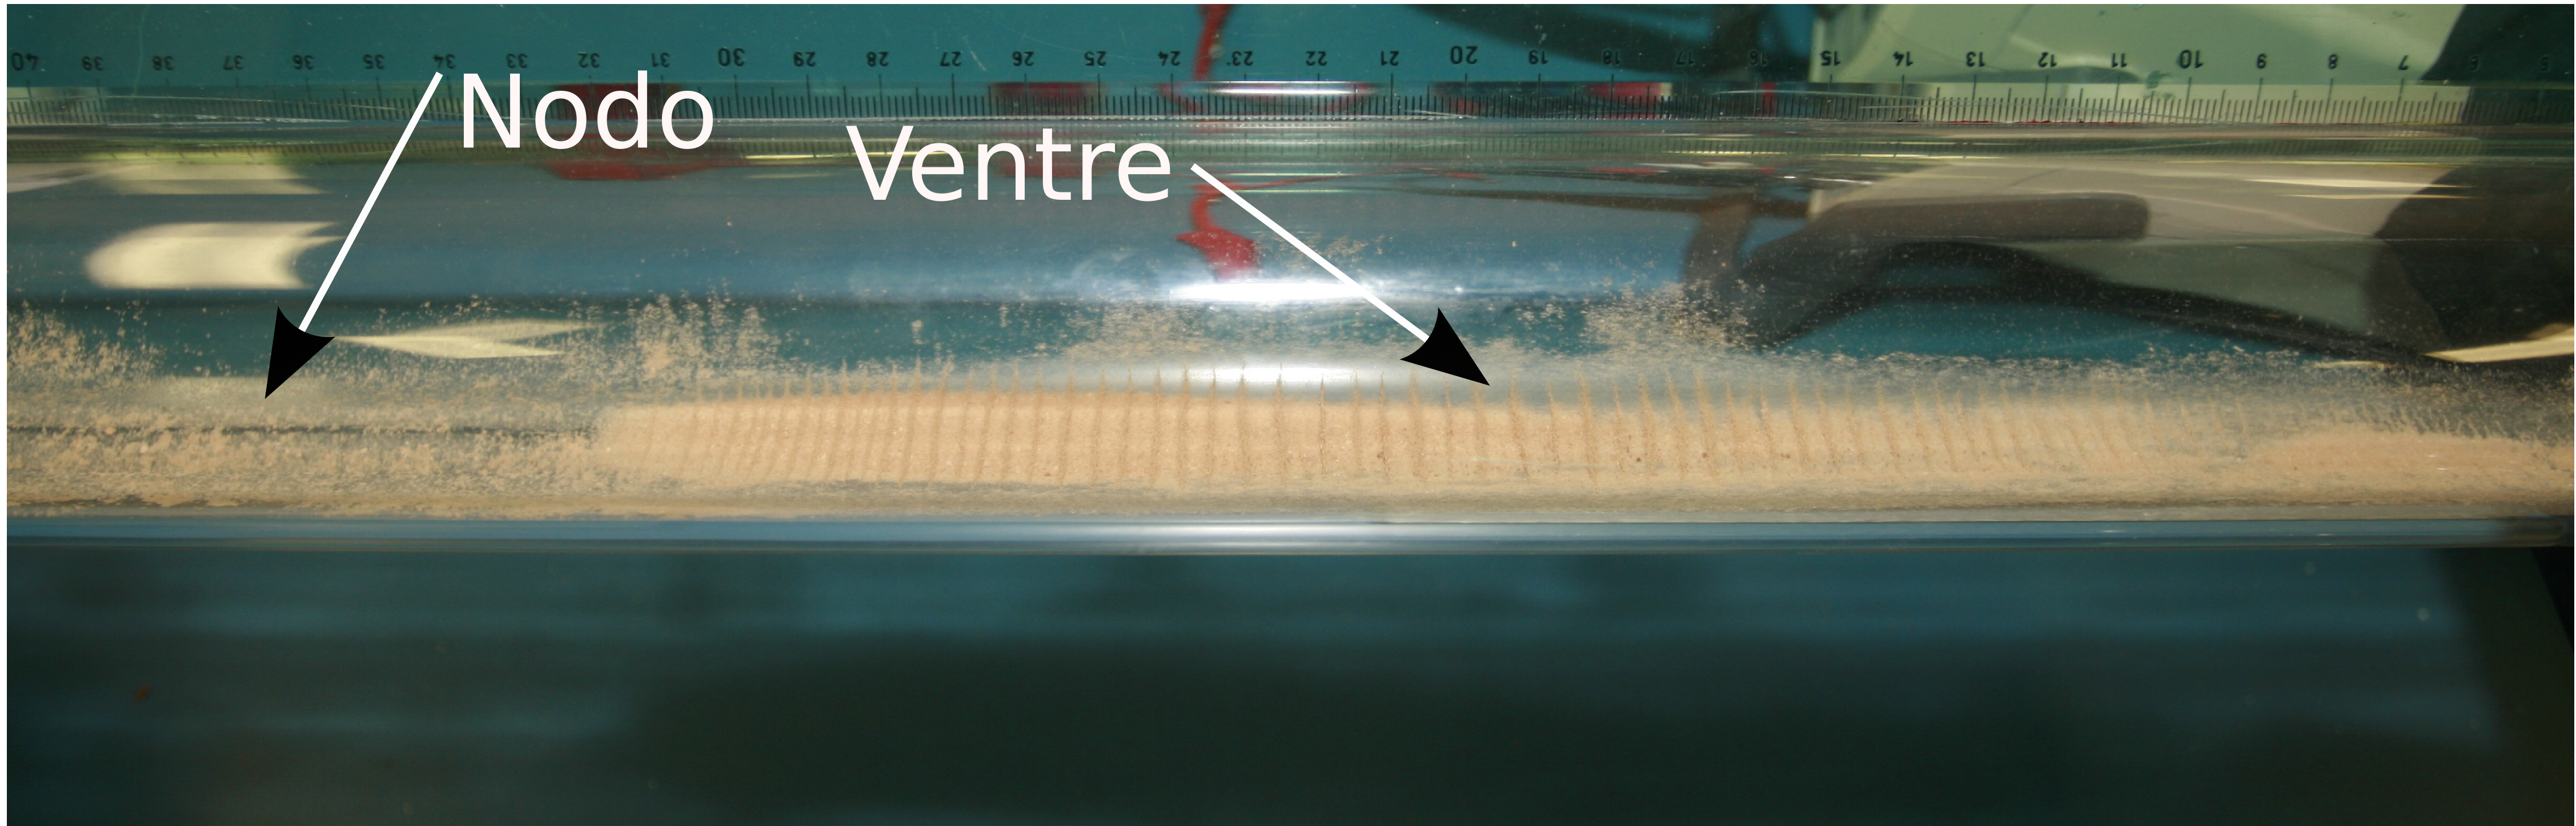
\includegraphics[width=\textwidth]{../Immagini/striature_1.png}
 % striature_1.png: 2145x577 pixel, 400dpi, 13.63x3.67 cm, bb=
 \caption{In prossimità dei nodi la polvere è immobile e l'ampiezza di oscillazione delle molecole d'aria non è sufficiente a mantenere i muri di polvere che possiamo osservare in prossimità dei ventri}
 \label{fig:striature_ventri}
\end{figure}


\section{Descrizione della strumentazione}

\subsection{Tubi opachi}
\begin{itemize}
 \item Tubo in cartone spesso che chiameremo \textbf{tubo 1} è corredato da un pistone con due microfoni che ci servirà per variarne la lunghezza
\item Tubo in cartone nero che chiameremo \textbf{tubo 2} è corredato da un pistone con un microfono per variarne la lunghezza
\end{itemize}

\begin{figure}[H]
 \centering
 \includegraphics[width=\textwidth]{../Immagini/tubi_cartone.jpg}
 % tubi_cartone.jpg: 3332x1090 pixel, 72dpi, 117.55x38.45 cm, bb=
 \caption{I tubi opachi in cartone come da una foto del laboratorio dell'anno scolastico 2008/2009}
 \label{fig:tubi_cartone}
\end{figure}


\subsection{Tubi trasparenti}
\begin{itemize}
 \item Tubo in vetro corredato da un pistone per variarne la lunghezza e imbuto per convogliare le onde sonore al suo interno
\item Tubo in plexiglas con tappo e imbuto per convogliare le onde sonore
\end{itemize}


\begin{figure}[H]
 \centering
 \includegraphics[width=\textwidth]{../Immagini/tubo_plexiglass.jpg}
 % tubo_plexiglass.jpg: 2838x1255 pixel, 72dpi, 100.12x44.27 cm, bb=
 \caption{Tubo in plexiglass per l'osservazione delle striature nella polvere, laboratorio anno scolastico 2008/2009}
 \label{fig:tubo_plexiglass}
\end{figure}


\subsection{Casse ed amplificatori}

\begin{itemize}
 \item 2 casse da $15W$ con impedenza di $8\Omega$
 \item 2 casse da $4W$ con impedenza di $4\Omega$
\item Un amplificatore in classe D (Yamaha D138) con una potenza RMS di $10W$ per canale
\end{itemize}

\subsection{Rilevatori e generatori}
\begin{itemize}
 \item 4 generatori di funzione
\item 2 oscilloscopi analogici da $20Mhz$
\item 2 oscilloscopi digitali con analizzatore di frequenza simulati tramite computer e scheda sonora
\end{itemize}

\section{Attività di laboratorio}
Vediamo ora nel dettaglio le attività che svolgeremo in laboratorio inziando dalla misura della velocità del suono.

\subsection{Misura della velocità del suono}
Per tale misura utilizzeremo i tubi in cartone e le casse non amplificate. Per prima cosa posizioneremo una cassa in prossimità di un'apertura del tubo ed inseriremo il pistone in quella opposta, quindi genereremo una frequenza sostenibile dalla cassa che misureremo accuratamente utilizzando l'oscilloscopio software. Dopo aver effettuato questi preparativi il sistema è pronto per le misure da eseguire in questo ordine:
\begin{itemize}
 \item Impostiamo l'oscilloscopio digitale in modalità analizzatore di spettro
 \item Spostiamo il pistone lungo il tubo fino ad incontrare una risonanza e riportiamo sul gambo dello stesso una tacca
 \item Ripetiamo il passo precedente fino ad estrarre il pistone dal tubo
 \item Misuriamo le distanze tra le tacche 
 \item Riportiamo in una tabelle la lista delle distanze misurate e la frequenza del suono
\item Ripetiamo tutta la procedura (compresa l'impostazione iniziale) per una frequenza diversa
\end{itemize}
Tutto il procedimento sopra descritto dovrebbe essere ripetuto per almeno tre frequenze diverse.

\subsection{Misura della lunghezza acustica del tubo}

Come sappiamo dalla teoria i tubi (e gli strumenti musicali) si comportano come se fossero leggermente più lunghi quando andiamo a calcolare le frequenze di risonanza. Vogliamo misurare di quanto dobbiamo correggere le nostre formule in funzione del diametro del tubo. Procederemo in questo modo:
\begin{itemize}
 \item Posizioniamo il pistone ad una distanza $L$ dall'estremo aperto del tubo e misuriamone accuratamente il valore
 \item Calcoliamo con la formula studiata un'armonica superiore per tale lunghezza del tubo (dobbiamo usare una frequenza abbastanza alta dato che le casse presenti in laboratorio non riproducono fedelmente le basse frequenze ad esempio possiamo usare la terza armonica oppure scegliere una $L$ sufficientemente piccola)
 \item Variando la frequenza in un intorno di quella calcolata cerchiamo esattamente la risonanza  e misuriamo accuratamente tale frequenza con l'oscilloscopio software del computer, la frequenza risonante dovrebbe essere più piccola di quella calcolata dato che il tubo è, dal punto di vista acustico, leggermente più lungo
\item Calcoliamo la lunghezza di risonanza teorica corrispondente a tale frequenza
\item Sottraiamo la lunghezza reale $L$ alla $L^*$ precedentemente calcolata per calcolare la correzione $\delta$.
\end{itemize}

Tutto il procedimento va ripetuto per almeno tre lunghezze diverse.

\subsection{Misura delle distanze tra le striature della polvere di sughero nei tubi trasparenti}

I tubi trasparenti e la polvere di sughero ci permettono una interessante visualizzazione delle onde stazionarie che si generano all'interno di un tubo. L'esperimento ci permetterà di osservare anche le caratteristiche striature che si formano quando la colonna d'aria è  in risonanza. 
Procedimento:
\begin{itemize}
 \item Misuriamo la lunghezza ed il diametro del tubo
 \item Disponiamo con l'apposito strumento un leggero velo di polvere lungo il tubo
 \item Disponiamo l'imbuto sull'imboccatura ed accostiamo la cassa.
 \item Cerchiamo le frequenza di risonanza del tubo (difficilmente si potrà osservare l'armonica fondamentale a causa delle caratteristiche meccaniche delle casse)
 \item Trascriviamo ogni frequenza di risonanza e fotografiamo le striature che si vengono a formare.

\end{itemize}

Tutto il procedimento va ripetuto sia con tubo semichiuso che con tubo aperto.
\begin{figure}[H]
 \centering
 \includegraphics[width=\textwidth]{../Immagini/tubo_grande_2/striature1.jpg}
 % striature1.jpg: 2486x616 pixel, 72dpi, 87.70x21.73 cm, bb=
 \caption{Striature nella polvere di sughero all'insorgere di una risonanza nella colonna d'aria all'interno del tubo di plexiglass.}
 \label{fig:striature1}
\end{figure}





\end{document}
